% Note to self: Compile using BibTeX (not Biber!) and pdflatex (not xelatex!)

\documentclass[11pt,a4paper]{article}
\usepackage[hyperref]{acl2020}

 % times is deprecated - using a modern times clone instead
\usepackage{mathptmx}

%\usepackage{titlesec}
%\titleformat{\section}{\normalfont\bfseries}{\thesection}{1em}{}

\usepackage{lipsum}
\usepackage{amsmath,amsthm,amssymb}
\usepackage{graphicx}
\usepackage{latexsym}
\usepackage{booktabs}
\usepackage{soul}
\renewcommand{\UrlFont}{\ttfamily\small}

\DeclareMathOperator*{\argmin}{argmin}

\newcommand{\havehair}{\texttt{have\_hair}}
\newcommand{\produceeggs}{\texttt{produce\_eggs}}

% This is not strictly necessary, and may be commented out,
% but it will improve the layout of the manuscript,
% and will typically save some space.
\usepackage{microtype}

\aclfinalcopy % Uncomment this line for the final submission
%\def\aclpaperid{***} %  Enter the acl Paper ID here

%\setlength\titlebox{5cm}
% You can expand the titlebox if you need extra space
% to show all the authors. Please do not make the titlebox
% smaller than 5cm (the original size); we will check this
% in the camera-ready version and ask you to change it back.

\title{PM Question Processing Final Project: 20 Questions}

\author{Wellesley Boboc \\
Universit{\"a}t Potsdam \\
Matriculation number: xxxxxx \\
\texttt{email@domain} \\\And
Anna-Janina Goecke \\
Universit{\"a}t Potsdam \\
Matriculation number: xxxxxx \\
\texttt{email@domain} \\\AND
Rodrigo Lopez Portillo Alcocer \\
Universit{\"a}t Potsdam \\
Matriculation number: xxxxxx \\
\texttt{email@domain} \\\And
Elizabeth Pankratz \\
Universit{\"a}t Potsdam \\
Matriculation number: 804865 \\
\texttt{pankratz1@uni-potsdam.de} \\}

\date{}

\begin{document}
\maketitle

\pagenumbering{arabic}

\begin{abstract}
lorem ipsum
\end{abstract}

\section{Introduction: Task and motivation}
\label{sec:intro}

Our task is to build a system that will play the game 20 Questions (20Q).
A human player will be able to think of a target object, and the system will strategically select questions that allow it to narrow down the candidate objects in its knowledge base.
It will incorporate the answers it receives and ultimately make a guess about what that target object could be.
If the target object that the human player has in mind is not already in its knowledge base, the system will add it in based on the information the user has provided.

This task is interesting and challenging because it not only involves generating natural-language questions to present to the human player, but also choosing which questions are the best ones to ask, and manipulating the knowledge representation in accordance with the answers that the human player provides.

So, on the one hand, the project contains the computational-linguistic subtask of question generation (given a feature in the dataset, generate a natural-language question asking about that feature to display to the user), and on the other, the engineering subtask of knowledge base manipulation.
For the latter, we will need to strategically select the best question to ask, incorporate the answers from the user as the game is played, and at the end, add previously-unseen objects into the knowledge base.

\section{Related work}
\label{sec:litreview}

We will briefly explore two areas in the literature that are relevant for our implementation: existing approaches to implementing 20Q, followed by rule-based question generation (QG).

\subsection{Previous 20Q implementations}
\label{subsec:prev20q}

Previous approaches to the implementation of a 20Q system have made use of diverse methods including probabilistic models \citep{DeyEa2019}, Reinforcement Learning (RL; \citealt{HuEa2018}), and variations of Artificial Neural Networks (ANNs; \citealt{ReddyEa2017, Burgener2006, ToninEa2018}).
The knowledge that the 20Q system has is often represented in a knowledge graph (KG; \citealt{DeyEa2019}), though some more sophisticated approaches also manage without \citep[e.g.][]{HuEa2018}.%
\footnote{A KG is essentially a graph where the nodes are entities and the edges between them are facts that connect them.
	For instance, a node \textit{Macron} might be connected to a node \textit{Paris} by the edge \textit{lives in} \citep[example from][]{GodinEa2019}, representing knowledge of the fact \textit{Macron lives in Paris}.}
Here, we will briefly discuss the relative merits of these implementations and how they inform our work on this project.

We begin with some probabilistic approaches.
In general, these are characterised by maintaining a probability distribution over the set of outcomes.
Consequently, none of the possible outcomes are ever totally discounted or thrown away---just associated with a lower probability.
%These are often associated with Bayesian-style updating, where the probabilities are computed anew after every time step.
This approach is good for situations in which the questions are answered by the users in a ``noisy'' way (e.g.\ when users answer inconsistently or wrongly).
In those cases, the system is still able to choose what the correct target object might be, even though the user has answered in a way that might seem incompatible with that object.

\citet{DeyEa2019} implemented a probabilistic model which operates on the dataset as weighted edge-node relations of a KG and updates throughout the course of the game. 
Here, the main idea of adjusting probabilities at every time step was exploited to generate a model that is able to predict the correct target object in fewer than twenty questions. 
Of particular interest is the way the model handles incorrect answers from the human player: the question generator does not fully reject or accept a certain object as being the target after every answer. f
Instead, it rebalances the probabilities at each step in the game. 
To identify the target object, the model categorizes the questions into two layers, a primary layer (wide range of objects) and a secondary layer (specific range, targeted towards a small set of objects). 
Even though the model has been proven to perform very well, i.e.\ half of the target objects could be identified in fewer than ten questions, their work is very limited in that it is designed to only apply to Bollywood movies. 
However, the use of KGs to create 20Q (probably adapted from graph format into a tabular database; see below) is an approach that we would like to pursue for our 20Q implementation, by further elaborating the ideas of \citet{DeyEa2019}, among others.

\citet{HuEa2018} also rely on a probability distribution over all objects which is then updated according to the answers.
However, their approach is different in that they use an RL framework: they implement a policy-based system of 20Q that uses reinforcement throughout the game. 
Instead of using a KG, the model for selecting questions is based on RL procedures trying to find the optimal reward function. 
%The questioner agent relies on a probability distribution over all objects which is then updated according to the answers.
\citet{HuEa2018} suggest a neural network that they call RewardNet which learns the immediate reward at each time step to improve the overall performance of the model, since only receiving a reward at the end of the game wouldn't allow the system to learn for each question.
The model continually improved its win rate over time and was shown to be able to identify the target object within 14 questions.
While this system clearly has excellent performance, incorporating RL into our project is not feasible; it is included in this literature review only for the sake of completeness.

Another approach that is probably too sophisticated for us, but nevertheless useful to know about, is the use of neural networks.
For example, \citet{ReddyEa2017} propose the application of KGs to generate sets of question-answer pairs within a Recurrent Neural Network architecture by deriving triple relations from given entities. 
The triples are composed of a subject, an object (both represented as nodes in the KG), and a predicate (represented as an edge in the KG). 
The model consists of two units: the \textit{Question Keywords and Answer Extractor}, which directly selects necessary information about an object from the KG, and the \textit{Natural Language Question Generator}, which is used as an encoder and decoder of the object's representation. 
Since this model has been able to outperform comparable approaches on question generation, we could consider adapting some of the assumptions, such as deriving the triple relations of the KG, for our project implementation. 

Perhaps the most widely-known implementation of the 20Q game is that of \citet{Burgener2006}, which can be found at \url{20q.net} and is also a popular toy. 
With more than 88 million plays, Burgener's implementation has a precision rate of 80\% when it asks twenty questions, and 95\% for twenty-five questions. 
The patent for the game describes the implementation of the deep ANN, which is structured as a matrix of target objects by questions. 
Each cell of the matrix contains an input-output connection weight, which defines the relationship between the questions/answers and the target objects. 
The network has two so-called modes: the first takes questions as input and targets as output, and the second takes target objects as input nodes and questions as outputs. 
The first mode maps answers to weights, while the second mode ranks questions. 
Similar to \citet{DeyEa2019}, target objects are prioritized, rather than filtered. 
This is a primary motivation for Burgener's choice of architecture, as it allows the model to correctly predict the target even when given incorrect or inconsistent answers, as mentioned above. 
As Burgener explains, it also allows the system to take into account cultural/demographic differences that may result in inconsistent answers about a given target object. 
This is a consideration we should also be mindful of in our implementation, as our proposed model operates on the assumption that the user is providing truthful answers (and that inter-user agreement would be high). 
The system of weights also allows for a more complex set of inputs than binary yes/no (e.g.\ sometimes, maybe, depends, rarely) where the degree of certainty of the answer is reflected in the weights used. 
While our immediate plan is to implement a binary answering system (or perhaps a three-way system, where ``unsure/unknown'' could also be an answer that would not contribute to the machine's prediction) as a proof of concept, keeping degrees of certainty in mind may help us to improve our final implementation.

Finally, \citet{ToninEa2018} describe another ANN implementation of the 20Q framework as part of a brain-computer interface to enable people with motor impairments to communicate. 
The system uses a weight matrix to store the strength of the connection between target statements and questions (where negative weights indicate that the expected answer to the question is no, and vice-versa for positive weights). 
After 15 questions, the model checks to see if there is only one target statement with a positive value. 
If there is no single positive value after twenty questions, the network returns the statement with the highest current value. 
When the network correctly estimates the target, the weight matrix is updated. 
We may want to adopt this sort of ``early checking'' threshold before a final guess after twenty questions. 
This paper also presents a very interesting example of how a 20Q implementation may have useful applications outside of the realm of games and entertainment.

\subsection{Rule-based Question Generation}
\label{subsec:qglit}

In the field of QG, one of the approaches to generating syntactically coherent questions is based on finding rules. 
In our project, we would like to follow this rule-based approach, most likely using the spaCy\footnote{\url{https://spacy.io}} library, as we saw in class.
This is because questions in 20Q are syntactically limited, so we do not need more complex approaches for this task.

An interesting approach to rule-based QG is the work of \citet{MhatreEa2019}, which is based on keyword modelling using Named Entity Recognition (NER) to generate questions from an input sequence. 
Each input sentence is preprocessed and parsed to resolve anaphoric reference. 
Thereafter, NER is used to identify the type of entity, which is important for the choice of \textit{wh}-component for the QG part of the model. 
Depending on the output of the NER procedure, the appropriate \textit{wh}-pronoun is chosen. 
One type of questions they create are yes-no questions, which is the type of question we will focus on.
To construct this kind of question, the authors simply perform subject-auxiliary inversion. 
Since this work makes use of the spaCy architecture, it is of particular interest for this project.
In the case of NER, spaCy is a widely used structure that provides a large range of entity types. 

\citet{KhullarEa2018} concentrate on rule-based QG using relative pronouns to achieve high syntactic accuracy and semantic suitability. 
Their system uses the spaCy dependency parser to evaluate the syntactic structure of sentences. 
Firstly, the input sentence is parsed to gain information about the presence of relative pronouns and about several linguistic features. 
Afterwards, this information is input to one rule within a predefined rule set to create the questions. 
The correct \textit{wh}-component is then determined according to these rules, resulting in a syntactically coherent question. 

Both of the above-mentioned systems are fascinating in that they consist of a simple structure by using spaCy's dependency parser and NER methods. 
By further elaborating on these approaches, we should be able to construct simple yet appropriate yes-no questions for our 20Q model.

\section{The knowledge base}
\label{sec:kb}

Our game uses a tabular knowledge base that contains 152 animals and 63 features for each object.
Each cell in the table is populated with a 1 or a 0 to indicate whether the given animal does or does not have the given feature.

We are currently developing the implementation on a preliminary knowledge base available \href{https://github.com/drdevinhopkins/20_Questions/blob/master/knowledge_base.csv}{here}.
It is a table consisting of 100 objects (mostly animals) and 28 features for each, and each cell in the table is populated with a 1 or a 0 to indicate that the given animal does or does not have the given feature.
For example, a subset of the knowledge base looks like this:

\begin{table}
\begin{center}
{\small \texttt{
	\begin{tabular}{lrrr}
		\toprule
		animal & have\_hair & feathers & produce\_eggs \\ \midrule
		aardvark & 1 & 0 & 0  \\
		antelope & 1 & 0 & 0 \\
		badger & 1 & 0 & 0 \\
		bass & 0 & 0 & 1 \\
		bat & 1 & 0 & 0 \\
		\bottomrule
	\end{tabular}
}}
\end{center}
\caption{The first five rows (instances) and three columns (features) in our knowledge base}
\label{tab:knowledge-base}
\end{table}

We compiled this dataset by combining a knowledge base with 100 animals and 50 features made available \href{https://github.com/drdevinhopkins/20_Questions/blob/master/knowledge_base.csv}{on GitHub} with ???.
\hl{[WELLESLEY: details about knowledge base construction]}

\section{Implementation}
\label{sec:impl}

We opted to implement a relatively deterministic decision-tree-based 20Q system, rather than a deep learning or reinforcement learning paradigm.
This was so that the inner workings of our system would remain transparent and everybody would be able to understand the code and work on improving it.
For those of us with an exclusively linguistic background, such a deep dive into deep learning or reinforcement learning felt like too much too soon.
This naturally means that our system is less sophisticated than it could have been if we had used a more modern paradigm, but on the other hand, its inner workings are also much easier to understand.
In the current section, we outline how we implemented our 20Q system (and see Section \ref{sec:limit} for some limitations of the chosen approaches).

\subsection{Feature selection}
\label{subsec:featselec}

The first question to tackle is ``How will the system decide which feature to ask about at each step?''
The basic motivation is to choose the most informative feature at each step, so that we narrow down the potential animals most quickly.
(We add some non-determinism later, so that it is not always the \textit{most} informative feature that is chosen at each step---this would make for boring gameplay---but first we focus on the basic mechanism for determining the informativity of a feature.)

We used a model in the style of a decision tree (DT) to tell us which feature is most informative at any given step.
A DT is ``defined by recursively partitioning the input space, and defining a local model in each resulting region of input space'' \citep[545]{Murphy2012}.
In our case, the input space consists of the knowledge base described above, and this knowledge base is recursively partitioned by each successive question that the system asks and the user answers.

In standard classification DTs, the space is split by the feature that minimises the entropy (i.e.\ maximises the information gain; \citealt{Quinlan1986}) in each partition.
However, that method is not applicable here.
That method requires an $n : 1$ mapping of instances to each class, which is the usual set-up in classification problems: one class contains multiple instances.
In our task, though, each individual object equates to a class (i.e.\ there's an \texttt{aardvark} class, an \texttt{antelope} class, and so on), so there is only one instance per class (but see Section \ref{subsec:out-of-db} below for handling of non-guessed animals that are not in the knowledge base).
The structure of our data makes our problem a non-typical classification task, so a different method must be used.

We chose to orient ourselves around the size of the two partitions of the input space that result from splitting on a given feature, and we select the feature that produces the partitions that are closest to each other in size.
To illustrate, say that we split on the first feature given in Table \ref{tab:knowledge-base} above, \havehair.
We would end up with one partition containing X animals that have no hair (i.e.\ where \havehair\ $= 0$), and another partition containing Y animals with hair (i.e.\ where \havehair\ $= 1$).

To see how even this split is, we take a ratio of these two numbers.
We want this ratio to be as close to 1 as possible, since that would represent a perfect split of our input space in half: $\frac{50}{50} = 1$.
This is because since we only have two values for each feature (yes or no, 1 or 0), consistently splitting our input space in half results in the highest information gain \citep[cf.][]{Quinlan1986, Bishop2006}.
%We selected this approach based on tree-based algorithms such as ID3 \citep{Quinlan1986, Bishop2006}.

So, for the feature \havehair, we get

$$\frac{|\havehair\ = 0|}{|\havehair\ = 1|} = \frac{X}{Y} \approx Z.$$

We call this value, $Z$, the \textsc{split cardinality ratio} (SCR) for the feature \havehair.
In general, the SCR for a feature $f$ is defined as in Equation \ref{eq:scr}.

\begin{equation}
SCR(f) = \frac{|f = 0|}{|f = 1|} 
\label{eq:scr}
\end{equation}

The best feature $f_{best}$ out of all features $f$ is the one for which the distance of the SCR from 1, i.e.\ $abs(1 - SCR(f))$, is closest to zero.
Formally, it is the solution to Equation \ref{eq:bestfeat}.

\begin{equation}
f_{best} = \argmin_f\ abs(1 - SCR(f)) 
\label{eq:bestfeat}
\end{equation}



%We illustrate this principle by also looking at the feature that actually minimises $abs(1 - SCR(f))$ in the current development dataset, \textit{Predator}:
%
%\begin{align*}
%	\frac{|Predator = 0|}{|Predator = 1|} &= \frac{45}{55} \approx 0.82 \\
%	\implies SCR(Predator) & = 0.82\\
%	\implies abs(1 - SCR(Predator)) &= 0.18.
%\end{align*}
%
%For \textit{Hair}, this value is $abs(1 - 1.33) = 0.33$, which is greater than $0.18$, so given the choice between these two features, our system would choose to split the input space on \textit{Predator} rather than \textit{Hair}.
%In question-processing terms, this means we would ask the user a question like ``Is it a predator?'' before asking ``Does it have hair?", as the former is more informative.

However, if we were to always choose $f_{best}$ to ask about at every step, the gameplay would be rigid and repetitive.
To make for a more varied gameplay, we decided to randomly sample a feature to ask about in proportion to its $abs(1 - SCR(f))$ score. 
This meant transforming the distribution over $f$ of $abs(1 - SCR(f))$ into a probability distribution, such that the features with the lowest $abs(1 - SCR(f))$ score would have the highest probability of being chosen at each step.
This means that any reasonably informative features are reasonably probable candidates.

To do this, we first transformed small values for $abs(1 - SCR(f))$, i.e.\ small distances from one, into large values, representing their greater probability of being chosen, by determining the maximum distance from one and subtracting every feature's distance from that (and adding one, so that the feature with that maximum distance value does not have a probability in the end of zero).
Then we scaled these transformed values into a probability distribution and sampled a feature from this distribution proportional to its probability.

This method does have certain drawbacks (see Section \ref{sec:limit}), but in addition to its simplicity, it also comes with one further advantage.
Even from the small subset of features shown in Table \ref{tab:knowledge-base}, it is apparent that the features are not independent.
For example, if you know that an animal has hair (i.e.\ \havehair\ $= 1$), you probably also know that it does not produce eggs (i.e.\ \produceeggs\ $= 0$).
So, an intelligent system should not ask about both of these features, since it should have gained the knowledge contained in both of them by asking about only one.
And, indeed, because of the way we bisect the database based on the features that best distinguish the animals still contained in it, we automatically avoid asking about highly correlated features.

For example, let us pretend that the five animals and three features in Table \ref{tab:knowledge-base} constitute the entire knoweldge base.
If we tell the system \havehair\ $= 1$, then it bisects the database and removes all animals with \havehair\ $= 0$.
However, since all animals with \havehair\ $= 0$ also have \produceeggs\ $= 1$, the feature \produceeggs now also only contains the value 0.
This makes it unsuitable as a feature to distinguish animals, so it will not be asked about in subsequent rounds.
(Even if two features are not perfectly correlated like these two are, after bisecting the data on one of them, the mixture of 0s and 1s in the other feature will be less even, so it will be less likely to be selected as a feature to ask about.)

\subsection{Guessing the animals}
\label{subsec:guess-animals}

Eventually, the gameplay will reach a point when the remaining animals in the pared-down knowledge base can no longer be distinguished by any of the features, since all the features will contain all 0s or all 1s.
At this point, the game moves on to the stage of guessing the animals that the user may be thinking of.

We were inspired by the approaches of \citet{DeyEa2019}, \citet{HuEa2018}, and \citet{Burgener2006}, who all maintain a probability distribution over outcomes that is updated over the course of the game based on the answers that the user provides.
The motivation behind this approach, as we mentioned above, is to improve the flexibility of the system, and in particular to not reject outright any outcomes that are incompatible with the user's answers.
Instead of removing these from the pool of potential answers immediately, their probability is simply reduced, but this means that they are still ``in the running'' to be guessed by our system, after it has guessed the higher-probability items.

Technically, the distribution that we maintain over animals is not a probability, since it does not sum to one; rather, it is a probability score that keeps track of how (in)compatible each animal is with the answers that the user has provided so far.
It can be thought of as bargain-basement Bayesian updating.

We initialise a uniform prior probability score of 20 (an arbitrary choice) across all animals at the beginning of the game and update it after each question based on the user's answers.
Specifically, we divide the current probability for each animal in half (also an arbitrary choice) if it is incompatible with the answer the user just gave.
Once the features have all been used up, we have a distribution of probability scores across animals that reflect how compatible they are with the user's answers.

The animals that are perfectly compatible with everything the user has entered have the same probability score that they started with; those that are incompatible with only one answer have half of the prior score, and so on.
Figure \ref{fig:bayesian-update} illustrates how this distribution changes over the course of a game.
At the end of the game, the system guesses the animals in decreasing order of probability.
For the example shown in Figure \ref{fig:bayesian-update}, it would guess \texttt{polar bear} and \texttt{hippopotamus} (the only ones with a probability score of 20), followed by the animals with a probability score of 10, and so on.

\begin{figure*}
	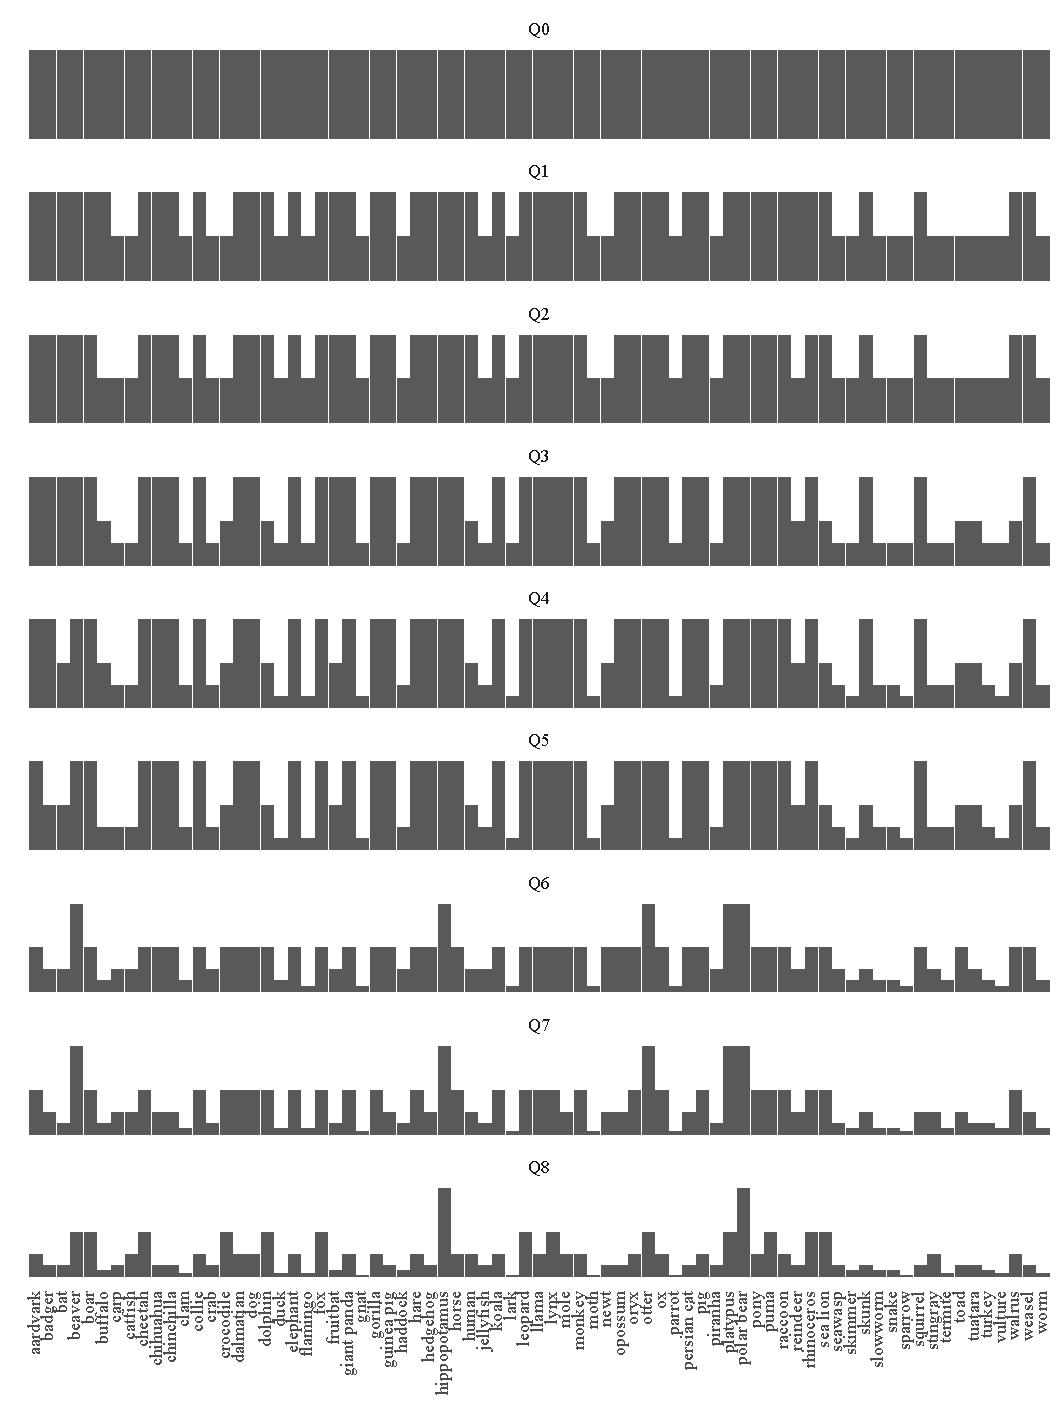
\includegraphics[width=\linewidth]{graphics/updating.pdf}
	\caption{Updating of probability scores across nine questions (only shown for a subset of 75 animals)}
	\label{fig:bayesian-update}
\end{figure*}

\subsection{Rule-based question generation}
\label{subsec:qg}

\hl{[ANNA]}


\subsection{Incorporating out-of-database objects}
\label{subsec:out-of-db}

\hl{[RODRIGO]}

``the perceived world is not an unstructured total set of equiprobable co-occurring attributes. Rather, the material objects of the world are perceived to possess (in Garner's 1974, sense) high correlational structure.
That is, given a knower who perceives the complex attributes of feathers, fur, and wings, it is an empirical fact provided by the perceived world that wings co-occur with feathers more than with fur'' \citep[29]{Rosch1978}

\vspace{\baselineskip}

\noindent The call graph in Figure \ref{fig:call-graph} provides a visual summary of how the functions in the \texttt{TwentyQuestions} class fit together.

\begin{figure*}
	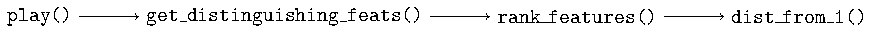
\includegraphics[width=.9\linewidth]{graphics/call_graph.pdf}
	\caption{Call graph of non-utility class methods in \texttt{TwentyQuestions}. Methods in (1) are for sampling features; (2) for asking users about features, getting user input, and taking the respective action; (3) for guessing animals; and (4) for the endgame and adding out-of-database animals}
	\label{fig:call-graph}
\end{figure*}

\section{Evaluation}
\label{sec:eval}

[introductory sentence]

\subsection{Win/loss rate}

\hl{[RODRIGO]}

\subsection{Quality of interpolated out-of-database items}

\hl{[RODRIGO]}

\section{Limitations}
\label{sec:limit}

\begin{itemize}
\item feature selection works by choosing the best feature for the remaining partition of the knowledge base, but if the animal that we're actually looking for does not get retained, then we don't end up asking questions that lead us to it; rather, we ask questions that are designed to lead us to some animal that is still in the partitioned knowledge base. This is somewhat saved by the probability score distribution across animals, but it is less likely in this case that the correct animal will be guessed.
\item Admittedly, this feature selection system does not learn to ask better questions over time; the method of choosing the best feature to ask about at a given time does not follow a strategy that extends beyond each individual turn.
We chose to focus our efforts on other parts of the project instead, since the current strategy already works quite well, and automatically deals with correlated features (see below).
If we were to develop the system further, though, this would certainly be a point of improvement, e.g. by learning from previous games which sequences of questions tend to perform well.
\end{itemize}

\section{Conclusion}
\label{sec:concl}

...

\bibliography{qp}
\bibliographystyle{acl_natbib}

\appendix

\section{Individual contributions}
\label{app:contributions}

All group members were in regular, active communication about ideas and directions in which to take the project.
It was a fully collaborative effort throughout.
We summarise here how we divided the workload between the four of us.

\paragraph{Wellesley} Literature work, prepared and held the in-class presentation, researched GUI and online server options, wrote and proofread sections of the project plan and the final paper.

\paragraph{Anna} Literature work, implemented the question generation, wrote sections of the project plan and the final paper.

\paragraph{Rodrigo} Implemented the handling of out-of-database items, conducted the evaluation, wrote sections of the final paper.

\paragraph{Elizabeth} Implemented the \texttt{TwentyQuestions} class and its core methods, wrote and proofread sections of the project plan and the final paper, hosted the GitHub repo, compiled \LaTeX\ files.

\end{document}
